
\section{Preliminaries}
Given $y_{it}$ an epidemic observation that have onset at time $t$ for location $i$, $y_{i,1:t}$ is the time series observations of the uni-variate surveillance. Due to the existence of backfill, each $y_{it}$ has its \textit{backfill sequence}\cite{kamarthi2021back2future} $y_{it}^{t:s}$ as of date $s$ ($s \geq t$). To be clear on nomenclature, throughout this paper, we use the term \textit{reference date} for date $t$ referring to the date when the observations have onset and the term \textit{report date} for date $s$ referring to the date when the observations are reported. 

For convenience, we introduce another term lag $l$ defined as $l = s-t \in \mathbf{N}$, which is the number of days between the report date $s$ and the reference date $t$. Now we change our notation henceforth and rewrite $y_{it}^s$ as $y_{itl}$. $y_{itl}$ is also named to be the $(l+1)$th release of $y_{it}$. The backfill sequence $y_{it}^{t:s}$ is equivalent to $y_{it,0:l}$. 



% TODO: Make the ticks larger
\begin{figure}
    \centering
    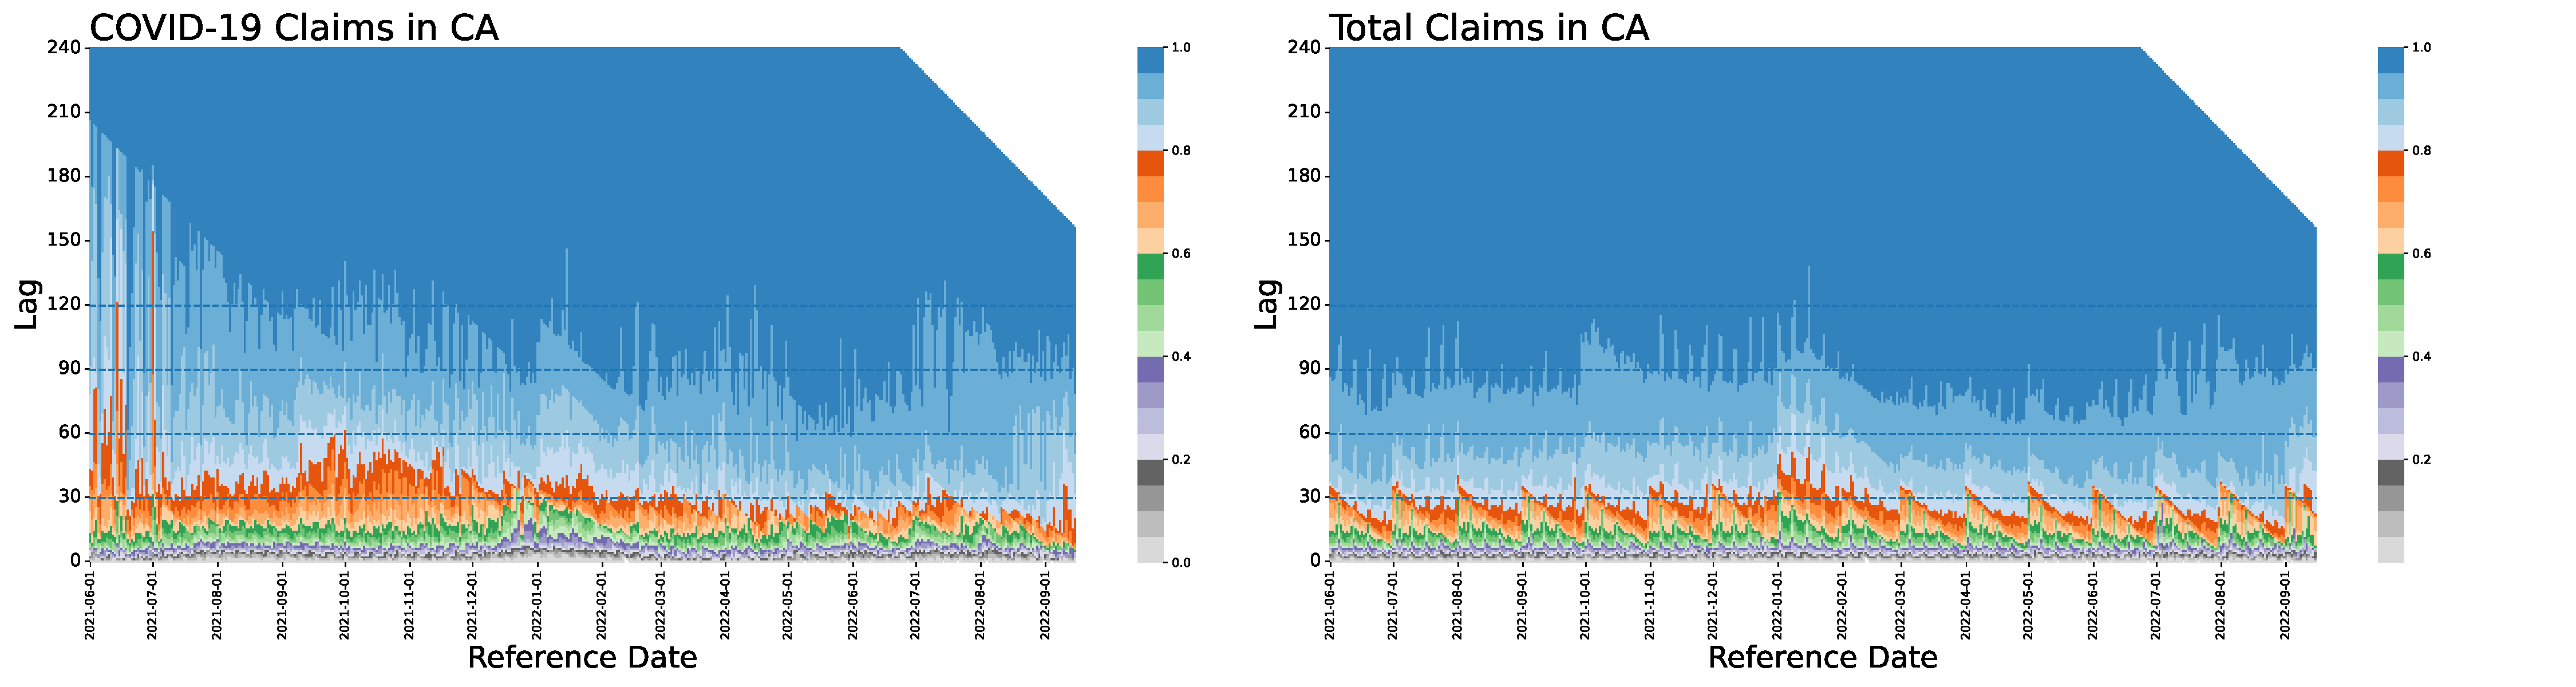
\includegraphics[width=\textwidth]{figs/completeness_CA.pdf}
    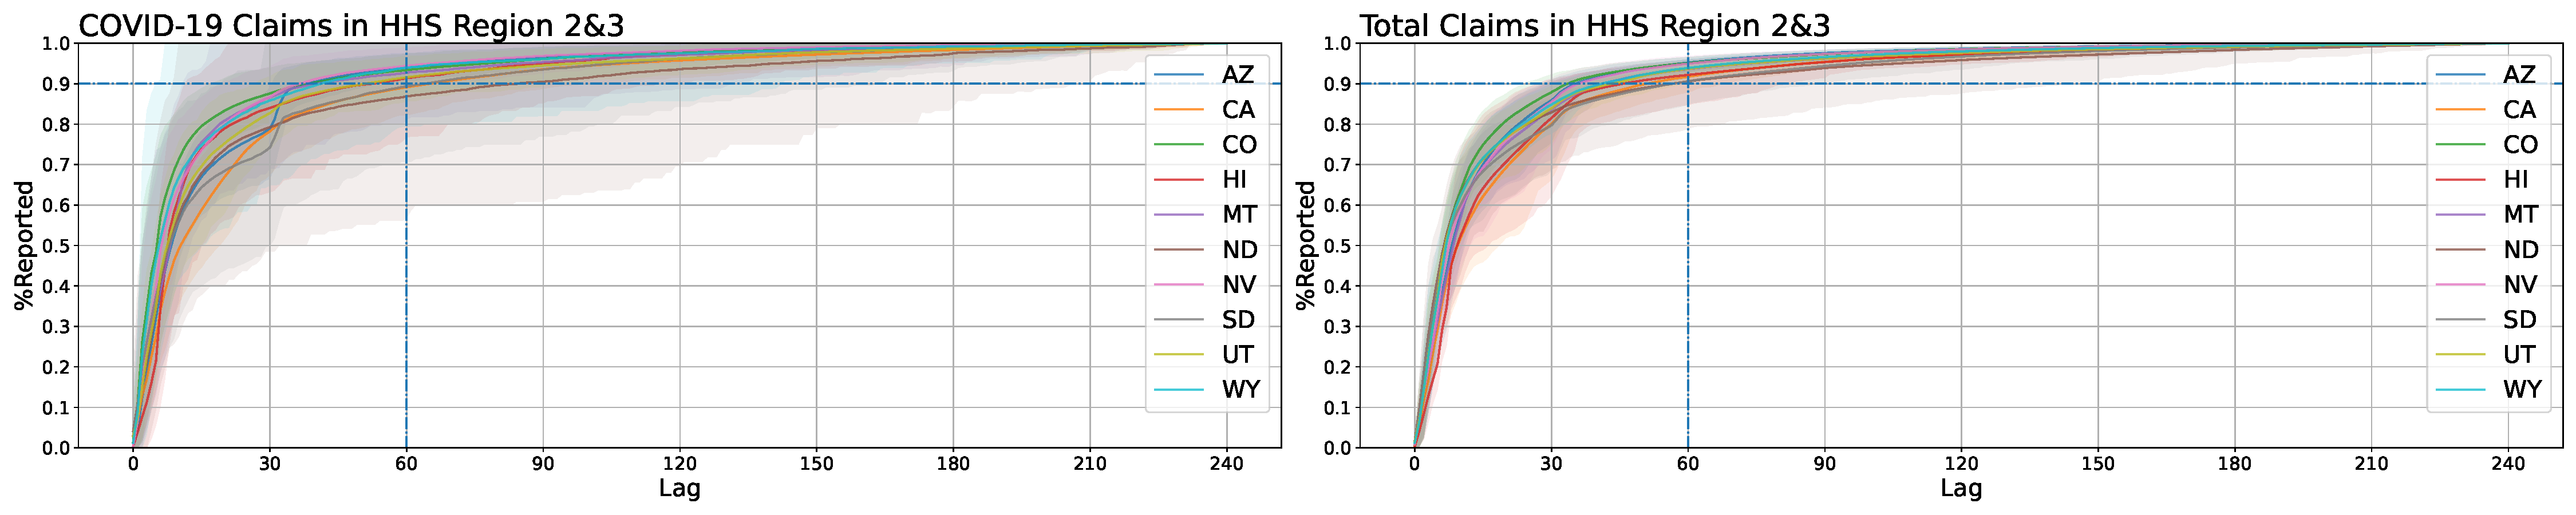
\includegraphics[width=\textwidth]{figs/completeness_lineplot_hhs8&9.pdf}
    \caption{\textit{Top: percentage of reported distribution in New York, grouped by lag, and recorded over reference dates. Bottom: Mean percentage of reported, averaged over all reference dates between 2021-04-01 and 2023-01-10, over lags for states in HHS Region 2\&3. The shaded bands correspond to 5\% quantile to 95\% quantile intervals. The left panel in the figure is based on CHNG outpatient COVID-19 claims data while the right panel is based on CHNG outpatient total claims data.}}
\end{figure}

Only a tiny part of data revisions occurs when data is lost but found later or when data is entered incorrectly but changed later. Most of them are caused by reporting delays. Therefore, the backfill sequence $y_{it,0:l}$ is guaranteed to converge to a particular value $Y_{it}$ when $l \geq L_{it}, L_{it}$ is sufficiently large. $Y_{it}$ is called the finalized value of $y_{it}$.

In this paper, we mainly use Change HealthCare (CHNG) 's insurance claims data which is available for more than two thousand most populous US counties, accounting for more than 45\% of the U.S. population in general. Multiple pre-processed signals based on this data are publicly available through Delphi's COVIDcast API \cite{reinhart2021open}. In order to construct the raw backfill data (including all historical versions), we start from the restricted line-level de-identified outpatient insurance claims data. It is worth pointing out that the data has geographic details down to 5-digit ZipCode level and is updated on a daily basis with no latency. We assume that a missing report is the same as reporting 0.

A useful way we propose to look at backfill pattern is by examining the variable $p_{itl}$ defined as $$p_{itl} = \frac{y_{itl}}{Y_{it}} \times 100\%$$
$p_{itl}$ describes the percentage of claims that have been reported after the $(l+1)$th release for location $i$ and reference date $t$. Since $Y_{it}$ is a theoretical value which is not obtainable directly, we use $y_{it}^s$ ($s$ = 2023-03-11) to approximate it. 

The distribution of $p_{itl}$ exhibiting how the backfill sequences vary over time. The day-of-week effect and week-of-month effect are evident, since the revision trends in lags for a fixed level of \%reported show spikes and bumps upward at the end of each week and around the beginning of each month. The reporting delay is prominent during the time period when the epidemic curve is at its peak. The top panel in Figure X displays results to this end using data in New York as an example. The backfill pattern is much more stable over time for total claims compared to COVID-19 claims. Overall, COVID-19 reporting is less efficient than Non-COVID-19 reporting. The variance is larger in the backfill pattern of COVID-19 claims which increases the diffculty in backfill correction. 

Furthermore, there is a high degree of heterogeneity in the backfill pattern across locations. For most of the locations (states and populous counties), the data revision tends to occur in the first two weeks of the backfill sequences to a large extent. The bottom panel in the figure shows that nearly all the mean \%reported of COVID-19 reaches 90\% when lag equals to 60 for states in HHS Region 2 and Region 3 except New Jersey. 


\subsection{Defining the Target}
Theoretically, the limit values of the backfill sequences are the target to be projected. However, the practice suggests that $L_{it}$ is highly inconsistent for different reference dates and can be incredibly large. Figure X gives an illustration where most of the states require more than 180 days (around half a year) for the backfill sequences of the COVID-19 claims reports with reference date=2021-08-01 to converge. If we set the projection target to be $Y_{it}$, we are forced to use the backfill sequences of $y_{it}$ with $t \leq s-L_{it}$ only for the training data on each testing date $s$. This means the backfill pattern captured based on the empirical distribution of all available data is very likely to be biased against the most recent backfill pattern, as discussed in the previous subsection. Note that, though $L_{it}$ is far from uniform at random, the distribution of \%reported indicates that substantial effective revisions are usually made within the first two months. Thus, we step back, setting a target lag $L$ and using $Y_{itL}$ as the projection target. For any location $i$ and reference date $t$, we assume that $$\mathbf{E}[\frac{Y_{itL} - Y_{it}}{Y_{it}}] \leq \epsilon $$ The larger the target lag $L$ is, the smaller $\epsilon$ can be. In short, the target lag $L$ selection faces a trade-off between timeliness and accuracy. Out of practical considerations and understanding of CHNG outpatient data, we set $L=60$ henceforth in our real-time backfill correction experiments.

\begin{figure}
    \centering
    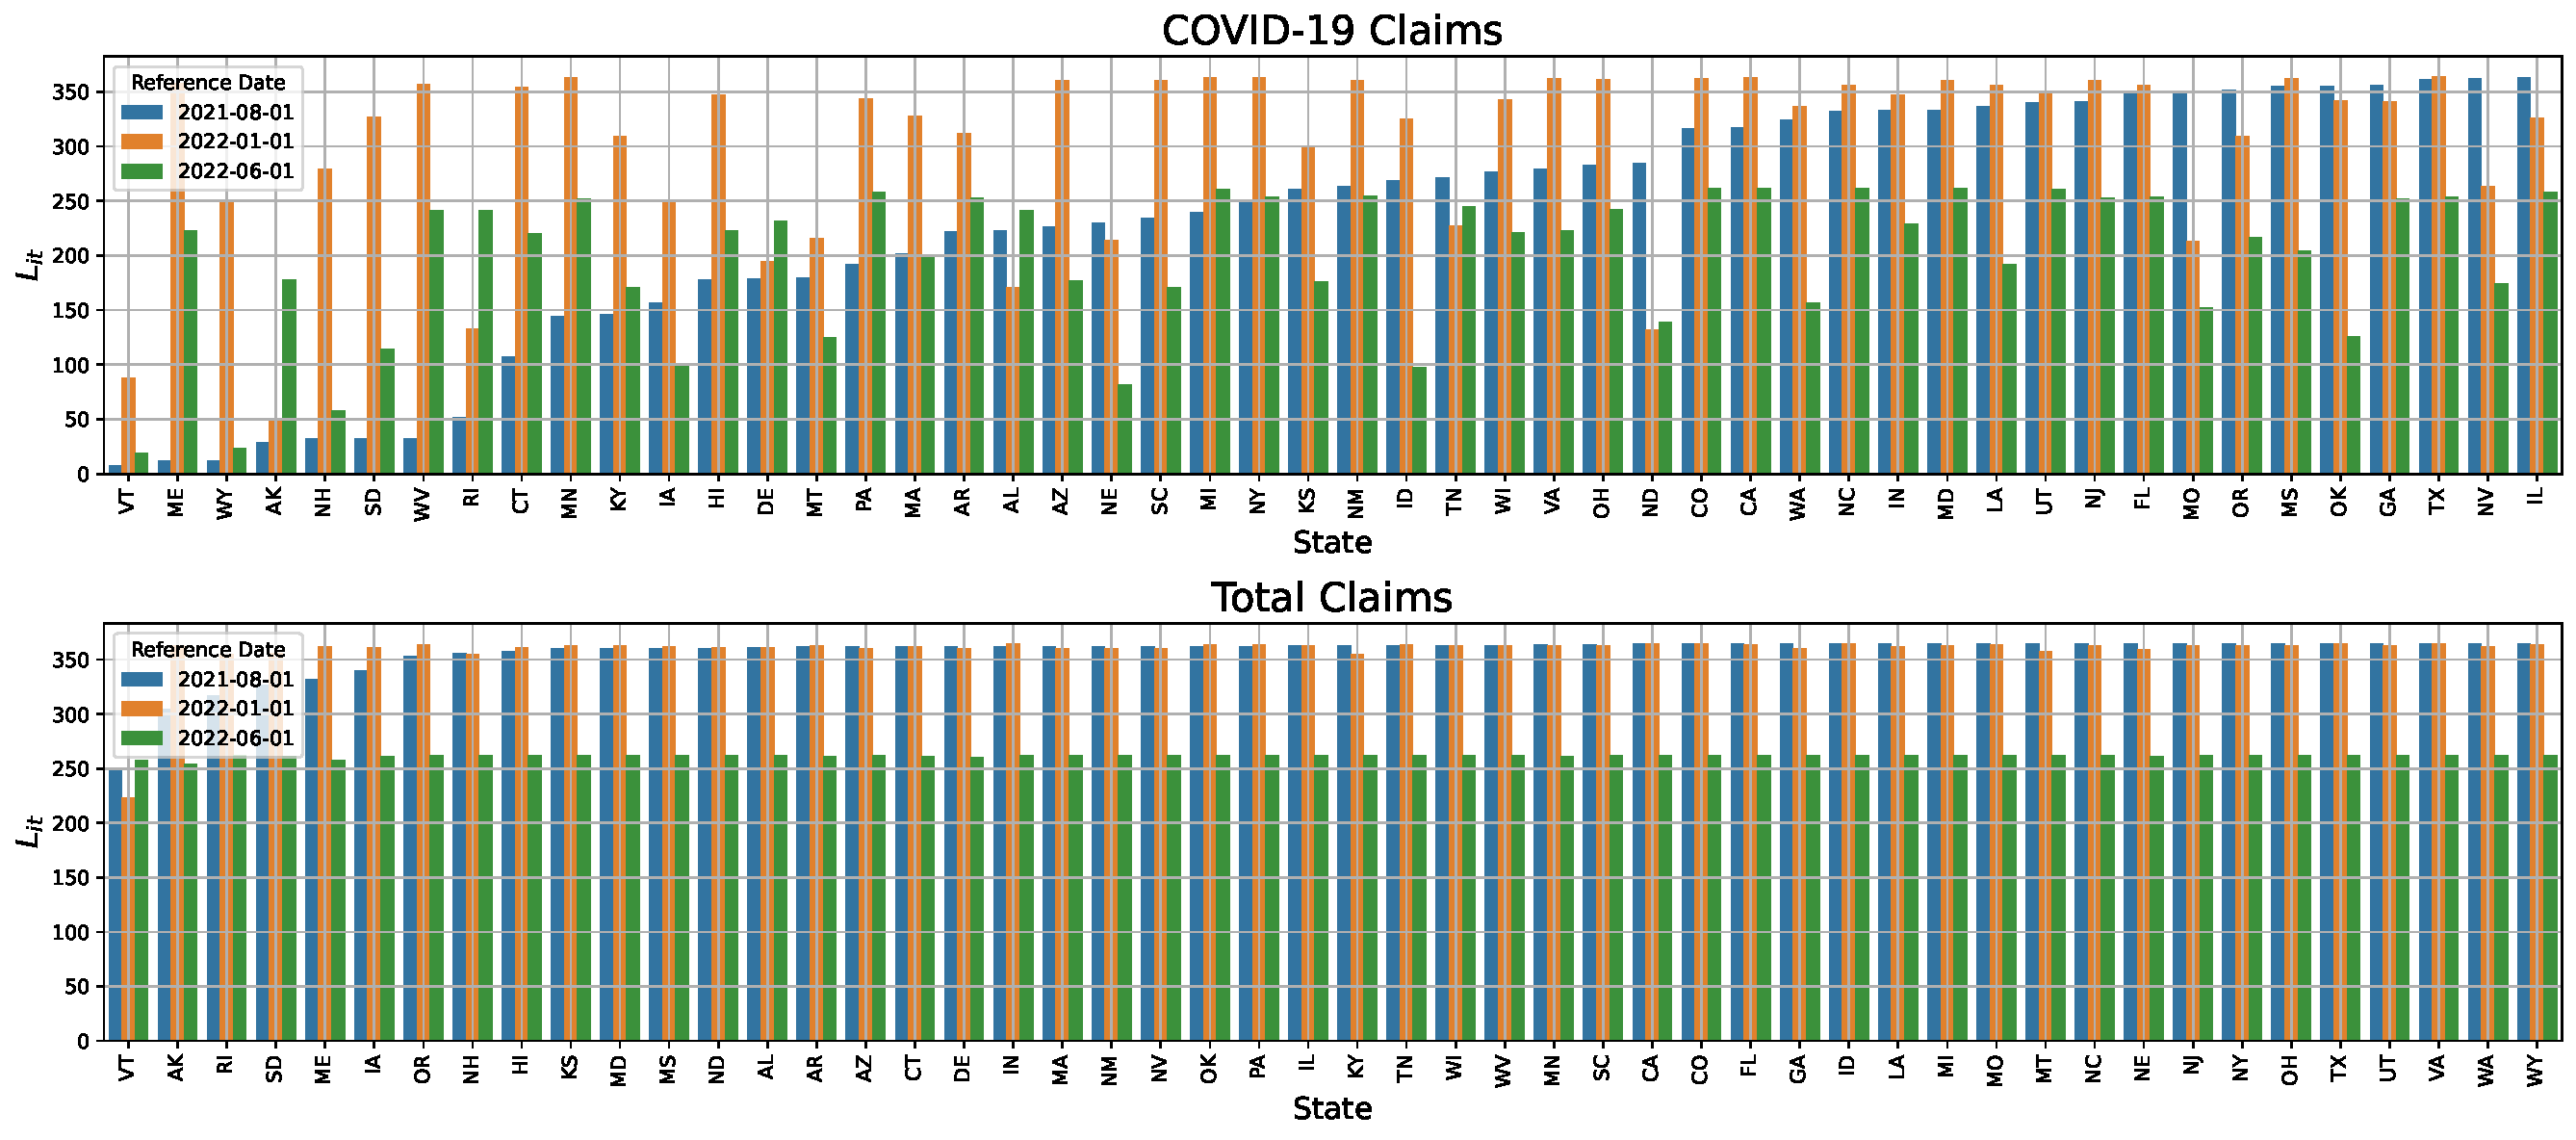
\includegraphics[width=\textwidth]{figs/Lit_examples.pdf}
    \caption{\textit{Top: comparison of the smallest lags required for convergence across states, displayed for a sample of different reference dates, based on CHNG outpatient COVID-19 claims data. Bottom: as in the figure on the top, but based on CHNG outpatient total claims data.}}
\end{figure}

\subsection{Problem Setup}
\textit{Estimation Period}. For every report day $t$ in between 2021-08-30 and 2023-03-11 inclusive (589 days in total), we make projections of the indicator values of reference dates $t, t-1, t-2, \cdots, t-(L-1)$ respectively based only on the data that would have been available as of time $t$. 

\textit{Geographic Scope}. We produce quantile projections for the targets of each reference date at state resolution and additionally produce the estimates for the top 200 populous U.S. counties. 

\textit{Evaluation}. We evaluate all the quantile projections in between 2021-06-01 and 2023-01-10 inclusive (589 days in total) and at each of the locations (50 states and 200 counties) against the target values as defined in section 2.1.

